\mysubsubsectionformatted{Eager vs Lazy Materialization}
\begin{center}
    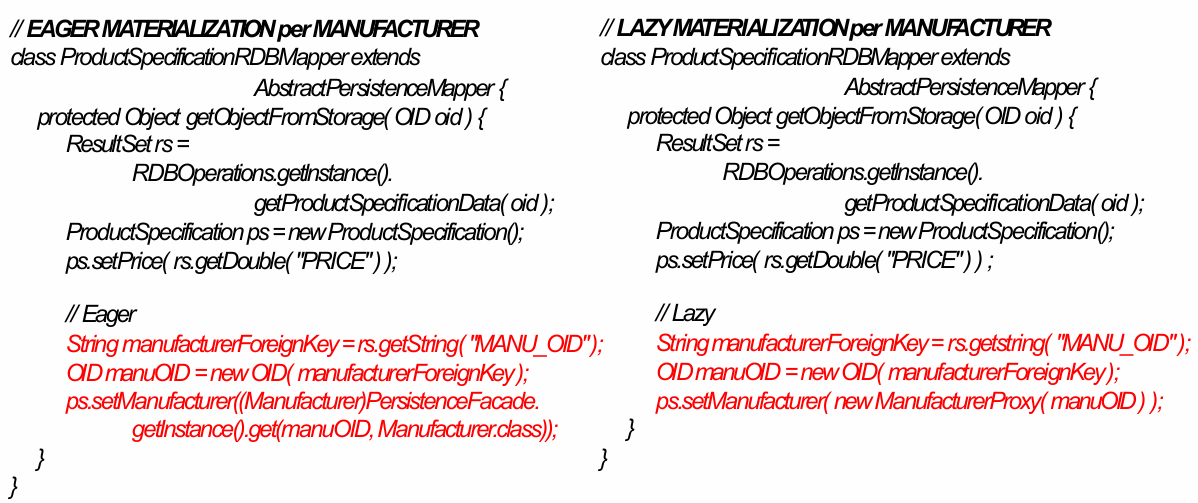
\includegraphics[scale=0.4]{Esercitazione - Design Patterns/Eager vs Lazy Materialization.png}
\end{center}

La differenza tra i due approcci sta nel caricamento in memoria del record in oggetto. Nel primo caso, avviene immediatamente
non appena i dati richiesti sono necessari, nel secondo caso il caricamento viene ritardato fino a quando l'oggetto non è
strettamente necessario.

Guardando il codice, entrambi gli approcci iniziano col prelevare la chiave\\ esterna del manifacturer, per poi creare un'ID da
associare all'oggetto (che verrà caricato in memoria) di quella chiave esterna (materializzazione: da record a oggetto).

\begin{enumerate}
    \item L'approccio \textbf{Eager} preleva direttamente l'oggetto Manufacturer \\dal database (\dots get(manuOID, Manufacturer.class))
    per poi settarlo al\\ Manufacturer oggetto.
    \item L'approccio \textbf{Lazy} agisce diversamente, crea prima un Virtual Proxy (ManufacturerProxy) dotato di identificativo
    unico (manuOID), settandolo nell'istanza di Manufacturer (ps). ManufacturerProxy rappresenta il sostituto di Manufacturer
    ma in formato più leggero e senza caricarlo in memoria direttamente.
\end{enumerate}